\chapter{Introduction}
\label{cha:intro}

% TODO: The first chapter contains a general introduction to the work. The goals are defined and the modus operandi is explained.

The mobile industry is without a doubt one of the most vibrant industries at the moment. It is characterized by rapid growth and intense competition which has led to fragmentation. 

This chapter give an overview of the evolution in the mobile device landscape, explain the problem of fragmentation and how cross-platform tools (CPTs) can solve this problem.

\section{The mobile device landscape}

Mobile phones have been around since the nineties and before but the smartphone as we know it now has only been around since the (nearly simultaneous) introduction of the iPhone 3G and the HTC Dream in 2008. In the last five years, smartphone sales have grown tremendously. According to quarterly studies by Gartner\footnote{Gartner, Inc. is the world's leading information technology research and advisory company \cite{Gartner}.} \citeGartner, smartphone sales have grown 544\% since the second quarter of 2008 (see \fref{fig:smartphone-sales}). Nowadays, smartphones are becoming ubiquitous and, in some regions like the United States, smartphone penetration has already reached more than 50\% \cite{Nielsen:2012}. 

\begin{figure}[h!]
    \begin{center}
        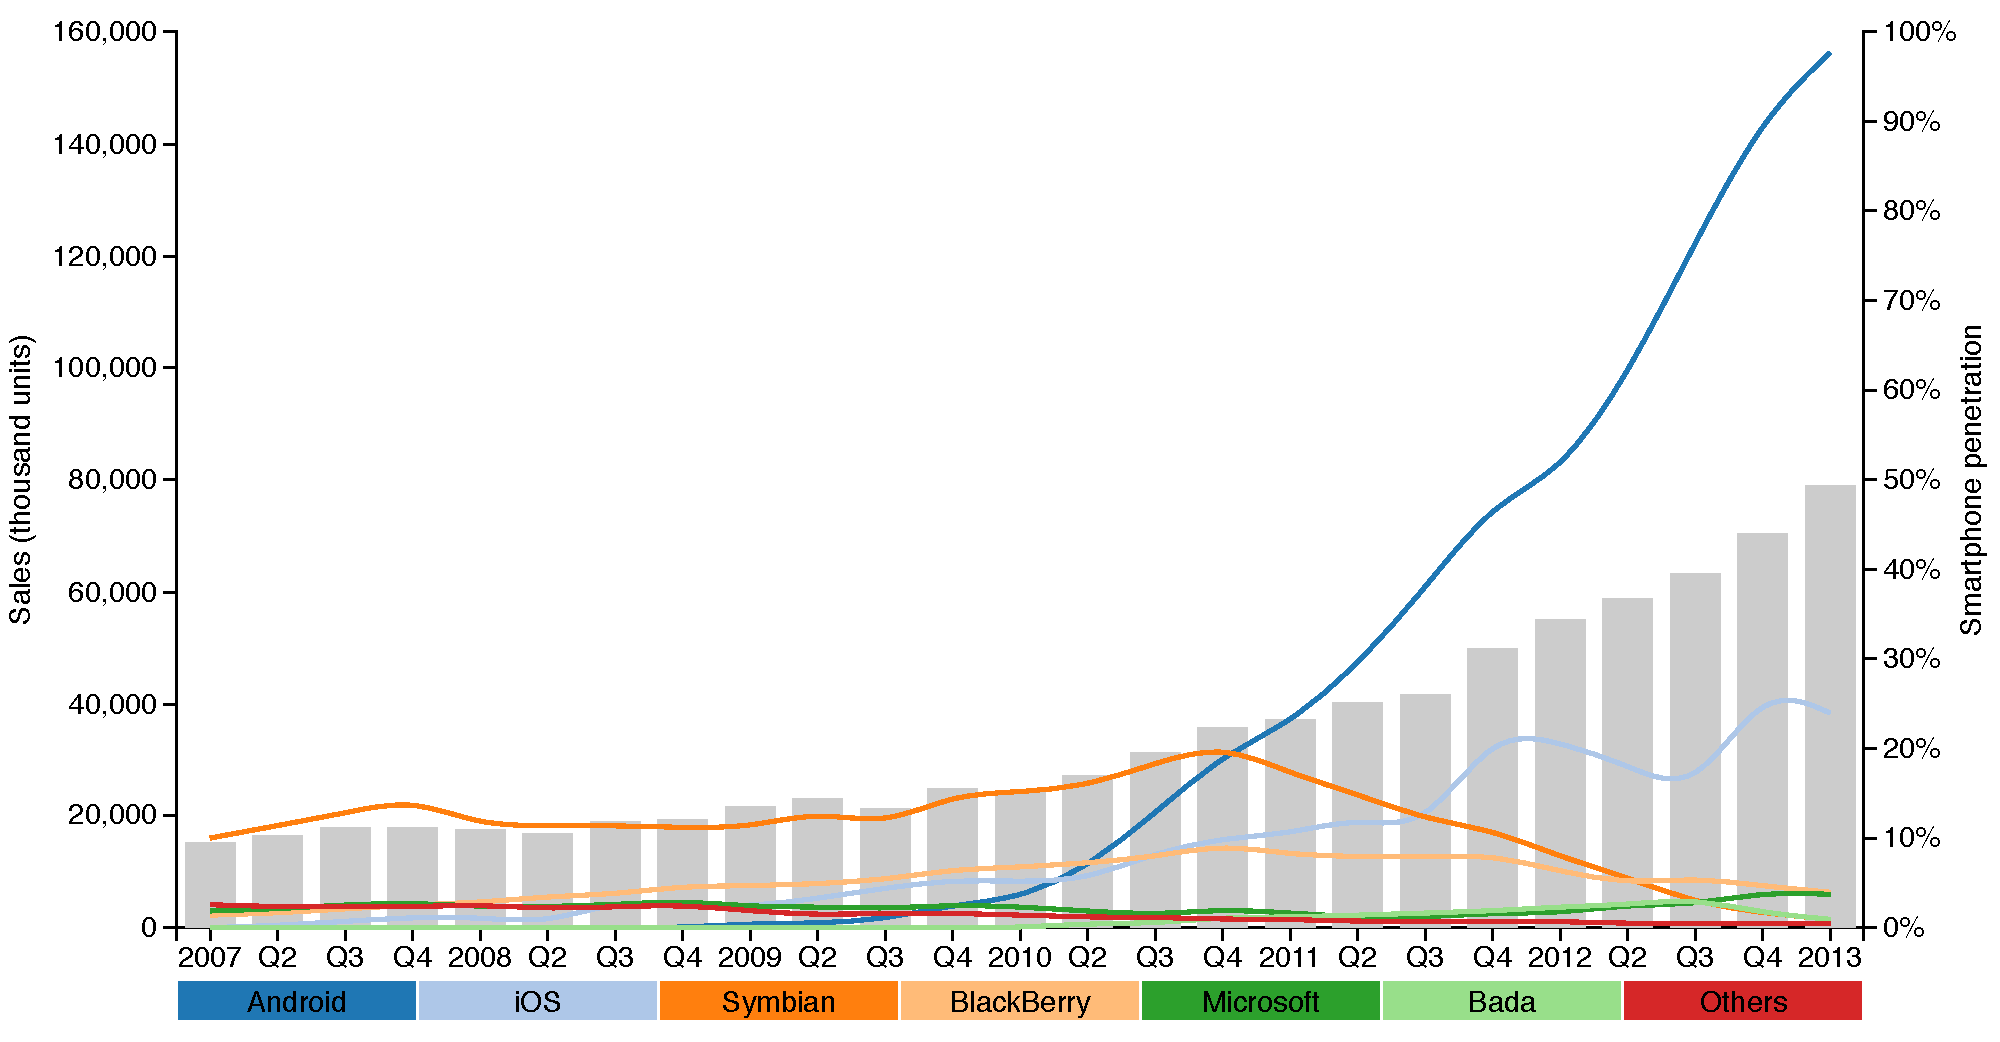
\includegraphics[width=\textwidth]{figs/smartphone_sales.pdf}
        	\caption{
        	    Growth of worldwide smartphone sales and smartphone penetration.\newline
        	    Source: Gartner \citeGartner
        	}
        	\label{fig:smartphone-sales}
    \end{center}
\end{figure}

\begin{figure}[h!]
    \begin{center}
        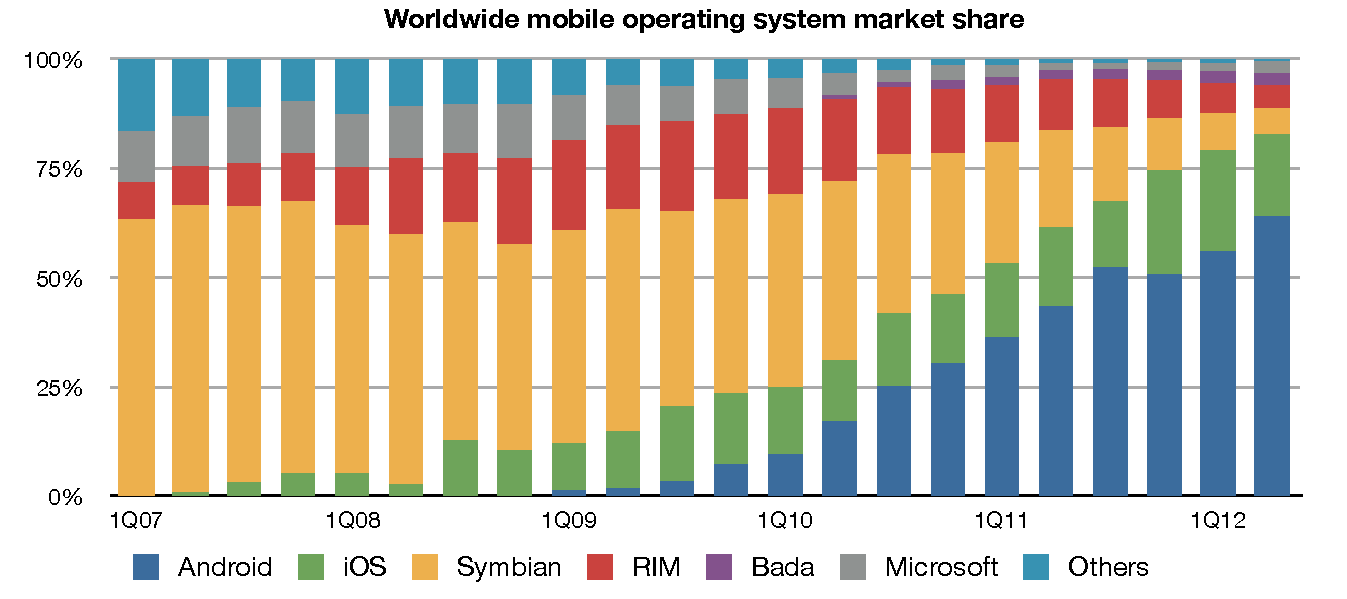
\includegraphics[width=\textwidth]{figs/smartphone_os.pdf}
        \caption{
            Growth of worldwide smartphone operating system market share.\newline 
            Source: Gartner \citeGartner
        	}
        \label{fig:smartphone-os}
    \end{center}
\end{figure}

\fref{fig:smartphone-sales} and \fref{fig:smartphone-os} also show that there is not a single major platform. The IDC\footnote{International Data Corporation is an American market research, analysis and advisory firm specializing in information technology, telecommunications and consumer technology.} predicts that there will be at least three major platforms covering 90\% of the worldwide smartphone market by 2016 \cite{IDC:phone}.

A similar scenario is playing in the tablet industry. According to other studies by both Gartner \citep{Gartner:11tab,Gartner:12tab} and the IDC \citep{IDC:tablet}, tablets will continue to gain popularity and sales will be mainly driven by iPads and Android tablets (see \fref{fig:tablet}).

\begin{figure}[h!]
    \begin{center}
        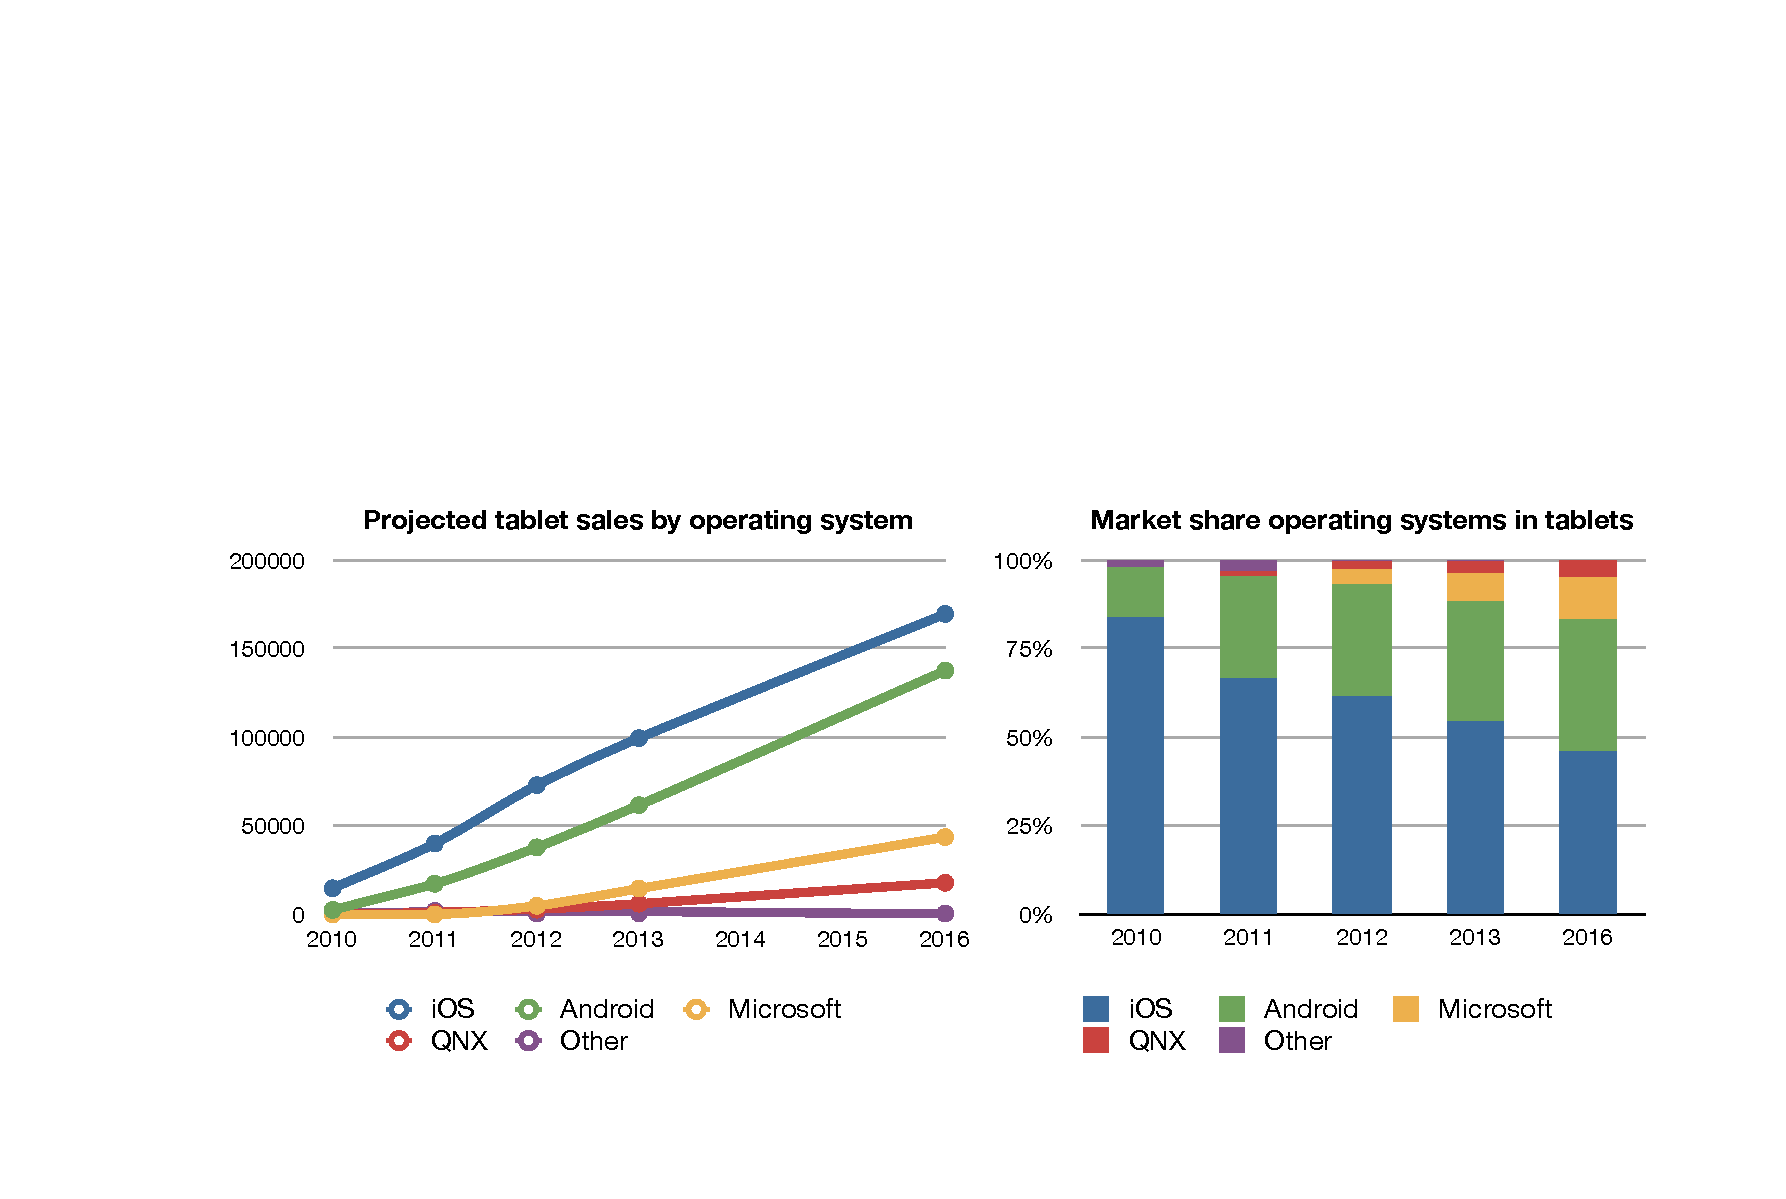
\includegraphics[width=\textwidth]{figs/tablet.pdf}
        \caption{
            Growth of worldwide smartphone sales and smartphone penetration.\newline
            Source: Gartner \citeGartnerTab
        }
        \label{fig:tablet}
    \end{center}
\end{figure}

Even though both companies do not agree on which platform will be the biggest by 2016, they both predict there will be at least three major platforms; iOS, Android and Windows. 

\section{The problem of fragmentation}

The competition among mobile device manufacturers has led to fragmentation on many levels. For consumers, fragmentation is usually a good thing. The more different devices there are, the easier it is for a consumer to pick one that fits his needs. 

For developers on the other hand, fragmentation is usually a bad thing because they will have to develop and test their applications on multiple devices to be able to guarantee the desired experience. This is expensive and time consuming.

From \fref{fig:smartphone-os} and \fref{fig:tablet} it is already clear that the market is divided by operating system or platform. This is platform fragmentation. But even within a single platform, there is fragmentation and it is multi-dimensional \citep{Kindel}.

% TODO elaborate on dimensions. You are stating something but you don't provide answers.

\subsection{Fragmentation on iOS}

iDevices (Apple devices running iOS) are available in different shapes and sizes but there are only a limited number of device configurations. This is why Apple can manage fragmentation quite well. 

For instance, iOS developers only have to support three \emph{logical} display resolutions: 480 by 320 (for all iPhones and iPod Touches until the iPhone 5 and iPod Touch 5G), 568 by 320 (for the iPhone 5 and iPod Touch 5G) and 1024 by 768 (for all iPads). Note that even though retina displays have four times the number of physical pixels, the logical resolution remains unchanged but the pixel density is doubled. 

Apple also provides good fitting mechanisms for applications that run on screens they are not designed for: on the iPad a ``2x'' button is available to make use of  all the screen real estate when running iPhone apps and on the iPhone 5 old applications are centered on the screen.

% TODO: runtime fragmentation

Overall, fragmentation is rather low on iOS.

\subsection{Fragmentation on Android}

Android is an open source platform and vendors are allowed to tailor it for their devices. As a result, there are hundreds of Android devices but also hundreds of Android flavours with different user interfaces as well. This leads to fragmentation in all dimensions.

Maintenance of such Android flavours is expensive and for this reason, manufacturers do not often provide updates for their devices. This has led to the notorious runtime fragmentation among Android devices (see \fref{fig:runtime_fragmentation}). 

\begin{figure}[h!]
    \begin{center}
        \label{fig:runtime_fragmentation}
        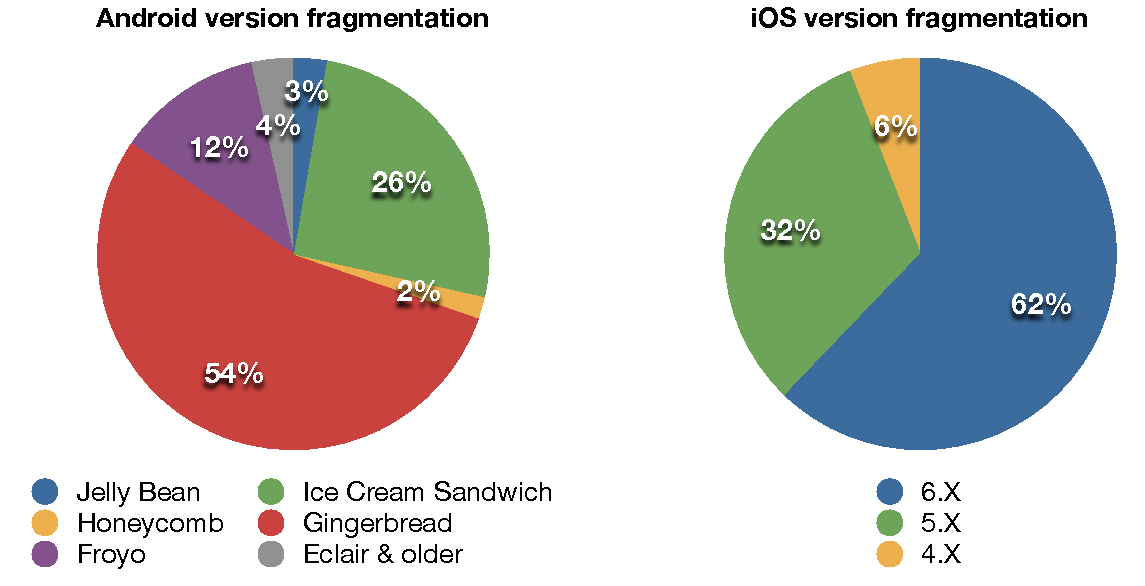
\includegraphics[width=0.8\textwidth]{figs/os_distribution.pdf}
        \caption{
            Runtime fragmentation for Android (data collected by Google during a 14-day period ending on November 1, 2012) \citep{android_distribution} and iOS (based on the statistics of developer David Smith) \citep{ios_distribution}.
        }
    \end{center}
\end{figure}

These flavours also contribute to user interface fragmentation. Large vendors often ship their devices with a custom user interface to make their product more unique. This results in a non-uniform user interface across Android devices.

Because of the sheer number of Android devices, there is also a sheer number of display resolutions and pixel density configurations which leads to a high display fragmentation. 

Overall, the Android platform is characterized by fragmentation in all dimensions.

\section{Cross-Platform Tools}

In the current economy, information is a company's most valuable asset and the rate at which information exchange takes place increases every day. Mobile Internet-enabled devices are a valuable resource for this purpose and, as a consequence, many companies want mobile applications for their businesses.

However, in an ever-changing and unpredictable industry like the mobile industry, it is very unwise to target a single platform. This could eventually lead to lock-in situations which companies try to avoid at all costs. Consequently, they will ask for a cross-platform solution. 

Cross-Platform Tools (CPTs) can help solving this problem. They reduce entry barriers (access to new platforms) and exit barriers (lock-in) by allowing developers to create cross-platform applications from a single codebase \cite{VMCPT:2012}. 

Cross-Platform Tools try to solve three major problems \cite{VMCPT:2012}: 

\begin{enumerate}
    \item \textbf{Fragmentation} The fragmentation issues described above are a pain for every developer. They need to test their applications on a large number of devices in order to be able to guarantee the desired user experience. A CPT can help to identify platform quirks and can provide workarounds. 
    \item \textbf{Access to new platforms and screens} Targeting a new platform is often hard. A developer needs to learn yet another SDK and/or programming language in order to deliver a working application. Using a CPT will drastically decrease learning time for new platforms.
    % TODO: AND SCREENS!
    \item \textbf{Development inefficiency} Maintaining codebases for multiple platforms is a difficult task. When using a CPT, all code is contained within a single codebase and no time is lost while synchronizing features and other maintenance tasks across codebases. 
\end{enumerate}

% TODO: finish Chapter


